\section{Durchführung und Aufbau}
\label{sec:Aufbau}
In \ref{fig:λ} ist ein prinzipieller Aufbau eines Interferometers gezeigt.
Für die Messungen der Wellenlänge wird jedoch die Apparatur aus Abbildung
\ref{fig:n} herangezogen und justiert.
Das Licht eines Diodenlasers wird durch das Interferometer geführt
und auf einer Photodiode zur Interferenz gebracht.
Ein Synchronmotor verschiebt über eine Mikrometerschraube einen Hebel und einen der Spiegel.
Der Hebel hat eine Übersetzung von $1:5,017$.
Die vorbeiwandernden Maxima werden von einem Zählwerk aufgezeichnet.
Dies wird fünf mal durchgeführt.
\\
Um den Brechnungsindex für Luft zu bestimmen wird die selbe Apparatur wie im
ersten Teil verwendet.
Zunächst wird Luft in die Messzelle hineingelassen und währenddessen werden die
vorbeilaufenden Maxima mit Hilfe des Zählwerks gezählt.
Um genauere Messungen zu erzielen, werden die Maxima beim Lufteinlass gemessen.
Danach muss die Zelle wieder entlüftet werden. Dieser Vorgang wird zehn mal
wiederholt.

\begin{figure}
  \centering
  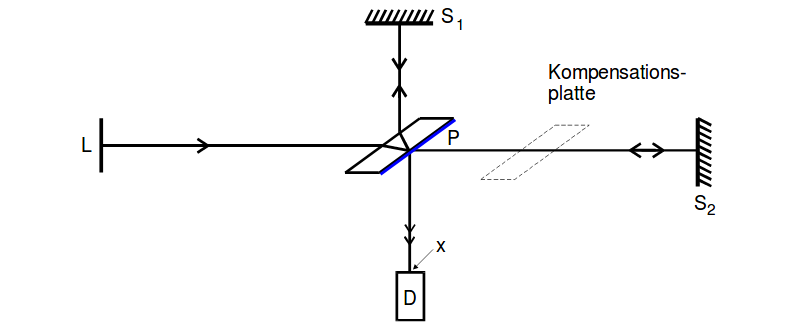
\includegraphics[width=10cm]{content/michelson_inter.png}
  \caption{Genereller Aufbau des Michelson-Interferometers\cite{Anleitung}.}
  \label{fig:λ}
\end{figure}

\begin{figure}
  \centering
  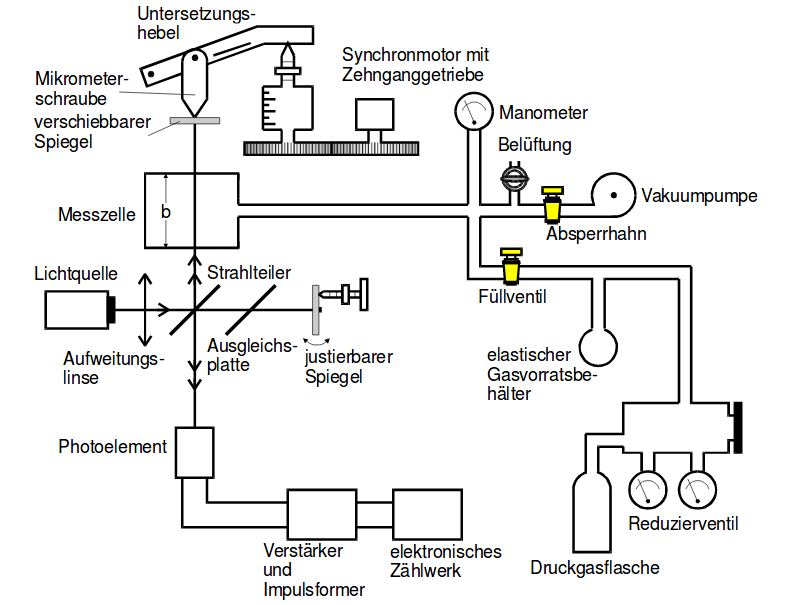
\includegraphics[width=10cm]{content/brechungsindex.png}
  \caption{Messapparatur für Wellenlänge und Brechungsindex\cite{Anleitung}.}
  \label{fig:n}
\end{figure}
